%% LyX 2.2.2 created this file.  For more info, see http://www.lyx.org/.
%% Do not edit unless you really know what you are doing.
\documentclass[12pt,twoside,magyar,twoside,rightopen]{report}
\usepackage[T1]{fontenc}
\usepackage[latin2]{inputenc}
\usepackage[a4paper]{geometry}
\geometry{verbose,tmargin=2cm,bmargin=2cm,lmargin=3cm,rmargin=2cm,headheight=12pt,headsep=24pt}
\usepackage{fancyhdr}
\pagestyle{fancy}
\setcounter{secnumdepth}{3}
\setcounter{tocdepth}{3}
\usepackage{verbatim}
\usepackage{amsmath}
\usepackage{amssymb}
\usepackage{graphicx}
\usepackage{setspace}
\onehalfspacing

\makeatletter
%%%%%%%%%%%%%%%%%%%%%%%%%%%%%% User specified LaTeX commands.
%\textwidth 160mm
%\oddsidemargin 0cm
%\topmargin -15mm
\usepackage{bm}
\lhead{}
\cfoot{}\rfoot{\thepage}
\renewcommand{\chaptermark}[1]{\markboth{\MakeUppercase{\thechapter.\ fejezet. #1}}{}}
\newcommand{\tg}{\mathop\mathrm{tg}}
\newcommand{\grad}{\mathop\mathrm{grad}}
\newcommand{\BME}{\hrule\vspace{6pt}{\large Budapesti M�szaki �s Gazdas�gtudom�nyi Egyetem\\
G�p�szm�rn�ki Kar\\
M�szaki Mechanikai Tansz�k}}
\newcommand{\szerzo}{G�ng� D�niel}
\newcommand{\konzulensek}{%
\hfill%
\parbox[t]{6cm}{\normalsize T�mavezet�:\\
\hspace*{3em}Zelei Ambrus\\
\hspace*{3em}tudom�nyos munkat�rs}}



\usepackage{babel}






\usepackage{babel}






\usepackage{babel}
\usepackage[style=numeric, backend=bibtex]{biblatex}
\addbibresource{irodalomjegyzek.bib} 

\fancyhf{}
\fancyfoot[CE, CO]{\thepage}
\fancyhead[RO]{\rightmark}
\fancyhead[LE]{\leftmark}
\renewcommand{\footrulewidth}{0.4pt}
\renewcommand{\sectionmark}[1]{\markright{\ \uppercase{#1}}}



\usepackage{babel}

\makeatother

\usepackage{babel}
\begin{document}

\title{\vspace{-5cm}
 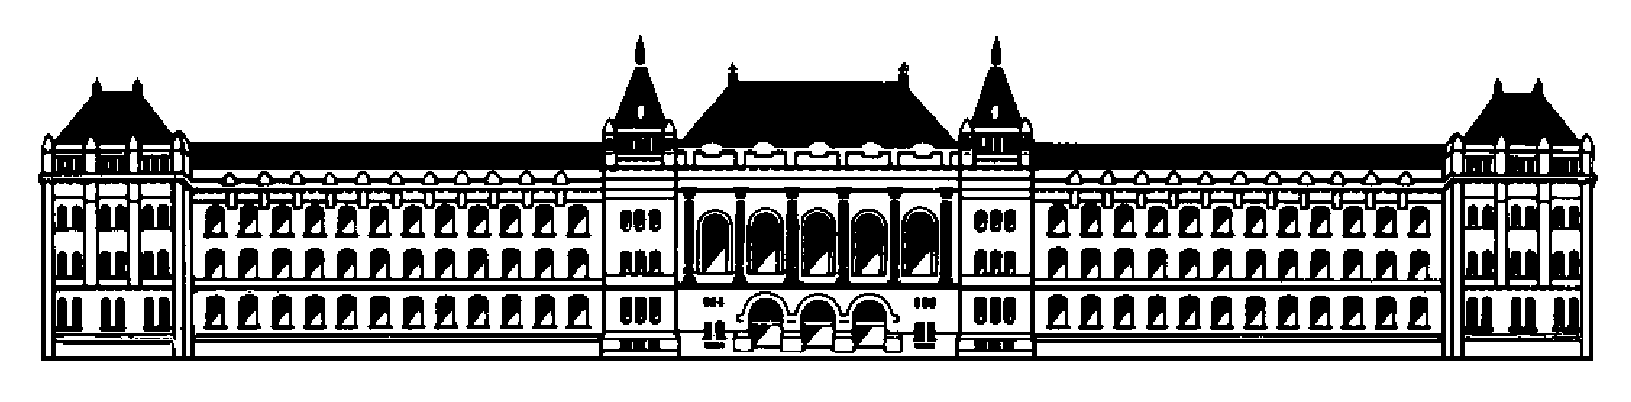
\includegraphics[width=0.4\textwidth,keepaspectratio]{bme_skyline}\\
 \BME\vspace{5cm}
 \\
 Szakdolgozat c�me\\
 ALULAKTU�LT RENDSZEREK SZAB�LYOZ�SI M�DSZEREINEK �SSZEHASONL�T�SA}

\author{K�sz�tette: \textsc{\szerzo}}

\date{\vspace{3cm}
 \konzulensek\\
 \vspace{4cm}
 Budapest, 2016}

\maketitle
\pagenumbering{roman}\thispagestyle{empty}

Szerz�i jog \copyright~\szerzo, 2016

\newpage{}\thispagestyle{empty}

\tableofcontents{}

\thispagestyle{empty}

\newpage{}

\chapter{Valami}

%\markboth{\MakeUppercase{Bevezet\H{o}}}{}%\addcontentsline{toc}{chapter}{Bevezet\H{o}}
\pagenumbering{arabic} \thispagestyle{empty}

\section{Garbage collector equation of motion}

Position vectors: 
\begin{equation}
\boldsymbol{r}_{0}=\left[\begin{array}{c}
x_{0}\\
y_{0}
\end{array}\right]
\end{equation}
\begin{equation}
\boldsymbol{r}_{1}=\left[\begin{array}{c}
x_{0}+l_{0}\cos(\varphi_{0}+q_{0})+\frac{l_{1}}{2}\cos(q_{1})\\
y_{0}+l_{0}\sin(\varphi_{0}+q_{0})+\frac{l_{1}}{2}\sin(q_{1})
\end{array}\right]
\end{equation}

\begin{equation}
\boldsymbol{r}_{2}=\left[\begin{array}{c}
x_{0}+l_{0}\cos(\varphi_{0}+q_{0})+l_{1}\cos(q_{1})+\frac{l_{2}}{2}\cos(q_{2})\\
y_{0}+l_{0}\sin(\varphi_{0}+q_{0})+l_{1}\sin(q_{1})+\frac{l_{2}}{2}\sin(q_{2})
\end{array}\right]
\end{equation}
Velocities: 
\begin{equation}
\boldsymbol{v}_{0}=\left[\begin{array}{c}
\dot{x}_{0}\\
\dot{y}_{0}
\end{array}\right]
\end{equation}
\begin{equation}
\boldsymbol{v}_{1}=\left[\begin{array}{c}
\dot{x}_{0}-l_{0}\dot{q}_{0}\sin(\varphi_{0}+q_{0})-\frac{l_{1}}{2}\dot{q}_{1}\sin(q_{1})\\
\dot{y}_{0}+l_{0}\dot{q}_{0}\cos(\varphi_{0}+q_{0})+\frac{l_{1}}{2}\dot{q}_{1}\cos(q_{1})
\end{array}\right]
\end{equation}
\begin{equation}
\boldsymbol{v}_{2}=\left[\begin{array}{c}
\dot{x}_{0}-l_{0}\dot{q}_{0}\sin(\varphi_{0}+q_{0})-l_{1}\dot{q}_{1}\sin(q_{1})-\frac{l_{2}}{2}\dot{q}_{2}\sin(q_{2})\\
\dot{y}_{0}+l_{0}\dot{q}_{0}\cos(\varphi_{0}+q_{0})+l_{1}\dot{q}_{1}\cos(q_{1})+\frac{l_{2}}{2}\dot{q}_{2}\cos(q_{2})
\end{array}\right]
\end{equation}
Angular velocities: 
\begin{equation}
\omega_{0}=\dot{q}_{0}
\end{equation}
\begin{equation}
\omega_{1}=\dot{q}_{0}+\dot{q}_{1}
\end{equation}
\begin{equation}
\omega_{2}=\dot{q}_{0}+\dot{q}_{1}+\dot{q}_{2}
\end{equation}
Kinetic energy: 
\begin{equation}
T=\sum_{i=0}^{2}\frac{1}{2}m_{i}\boldsymbol{v}_{i}^{2}+\frac{1}{2}\theta_{i}\omega_{i}^{2}
\end{equation}
Center of mass: 
\begin{equation}
\boldsymbol{r}_{C}=\frac{m_{0}\boldsymbol{r}_{0}+m_{1}\boldsymbol{r}_{1}+m_{2}\boldsymbol{r}_{2}}{m_{0}+m_{1}+m_{2}}
\end{equation}
\begin{equation}
\boldsymbol{v}_{C}=\frac{m_{0}\boldsymbol{v}_{0}+m_{1}\boldsymbol{v}_{1}+m_{2}\boldsymbol{v}_{2}}{m_{0}+m_{1}+m_{2}}
\end{equation}


\chapter{v�ge}

\begin{comment}
\bibliographystyle{plain}
\addcontentsline{toc}{chapter}{\bibname}\bibliography{irodalomjegyzek}
\end{comment}
\nocite{*}
\printbibliography[ heading=bibintoc, title={Irodalomjegyz�k} ]


\appendix
%dummy comment inserted by tex2lyx to ensure that this paragraph is not empty%dummy comment inserted by tex2lyx to ensure that this paragraph is not empty%dummy comment inserted by tex2lyx to ensure that this paragraph is not empty%dummy comment inserted by tex2lyx to ensure that this paragraph is not empty

\chapter*{F�ggel�k}

\addcontentsline{toc}{chapter}{F�ggel�k} \setcounter{chapter}{6}
%\setcounter{equation}{0} % a fofejezet-szamlalo az angol ABC 6. betuje (F) lesz \numberwithin{equation}{section} \numberwithin{figure}{section}

\end{document}
